\documentclass[11pt]{article}
\usepackage[margin = 1.4in]{geometry}
\usepackage{tikz}
\usepackage{pgfplots}
\usepackage{amsmath}
\usetikzlibrary{patterns}

%opening
\title{Computing the Moments of Inertia of Spinning Bodies Accelerated by Falling Masses}
\author{Andreas Badea}
\date{\today}


\begin{document}

\maketitle

\begin{center}
	\begin{tabular}{l r}
		Date Performed: & November 3, 2017 \\ % Date the experiment was performed
		Partners : & Eashwar Mahadevan \\
		& Lindsay Nottingham \\
		Instructor: & Dr. Bradley Miller % Instructor/supervisor
	\end{tabular}
\end{center}

\section{Introduction}
The moment of inertia of some body quantifies that body's resistance to an angular acceleration. Any object will tend to keep its velocity constant provided no external force acts upon it and causes an acceleration. This is simply inertia as described by Newton's first law of motion. However, forces do tend to act on objects, and it is useful to be able to describe how an object's velocity will change function of some force acting upon the object. This is not particularly difficult to do. One may, without much difficulty, conclude that a body will accelerate more as a larger force acts upon it, and that a body will provide a greater resistance to acceleration if it has a larger mass. This relationship is quantified in Newton's second law of motion, 
\begin{equation}
a \propto \frac{F}{m} \label{EQ:1}
\end{equation}
The very same relationship occurs with regards to rotational motion. That is, firstly that rotating objects have inertia. An object in rotation will tend to continue rotating just as a linearly moving body will continue to move with the same velocity. Likewise, a torque acting upon a body will impart an acceleration. However, a rotating body's mass is not necessarily directly proportional to its resistance to rotational acceleration. This quantity is called a moment of inertia and is denoted by the symbol \(I\). If one uses this information to create an analogue of the expression in equation \eqref{EQ:1}, one is left with the expression 
\begin{equation}
\alpha \propto \frac{\tau}{I}
\end{equation}
This resistance to angular acceleration, this moment of inertia is distinct from mass because it depends on the distribution and placement of the mass within the spinning object. If the mass of an object is concentrated close to the axis of rotation, inducing an angular acceleration is much easier than if the mass of the object is concentrated farther away from the center. The moment of inertia of a single point is proportional to the mass of the point multiplied by the square of the distance between it and the axis of acceleration.
\begin{equation}
	I = m r^2
\end{equation}
For more complex masses one may simply sum the moments of inertia of each of the points within the complex figure.
\begin{equation}
I = \int r^2 \mathrm{d}m
\end{equation}
However for even more complex solids, solids that perhaps even exist in the physical world, one may, in place of using the geometry of figure, compute the moment of inertia by actually applying some quantifiable toque on the body and measuring the angular acceleration that the torque induces in the spinning object. The following experiment will serve as a method for computing the moment of inertia of a spinning body accelerated by the constant toque of a falling mass. And will serve to confirm that a body's resistance to acceleration is indeed proportional to the sum its mass and to the square of the distances to the axis of rotation.
  
\section{Procedure}
The experiment was divided into two portions. In the first, two masses were placed on a metal rod such that the center of their masses remained 10cm from the center of the rod. The masses were held in place by two wing nuts. The center of this rod was suspended on the top of a second vertical rod which was permitted to rotate. This entire apparatus, the two rods, the masses suspended at a constant distance from the axis of rotation, and the wing nuts holding the masses in place, was the rotating mass whose moment of inertia intended to be found. The constant torque applied to the apparatus was supplied by a falling mass. A long string was positioned with one end wrapped around the circumference of the vertical rod the center passing through a small pulley and the opposite end with a small mass allowed to dangle above the ground. As the mass would begin to fall it would pull on the rod and the whole apparatus would begin to spin. The mass of the individual masses on the rod was permitted to vary throughout the experiment while the distance to the center was fixed at 10cm.
In the second experiment, the only 200 grams were ever placed on either ends of the rods, but the distance at which they were placed was permitted to vary between 15cm and 3cm.

The time for the masses to traverse the distance between the tabletop on which the apparatus was placed and the floor was measured and will be used to compute the acceleration at which mass falls and eventually the moment of inertia of the spinning object. 

\begin{figure}
	\centering
	
	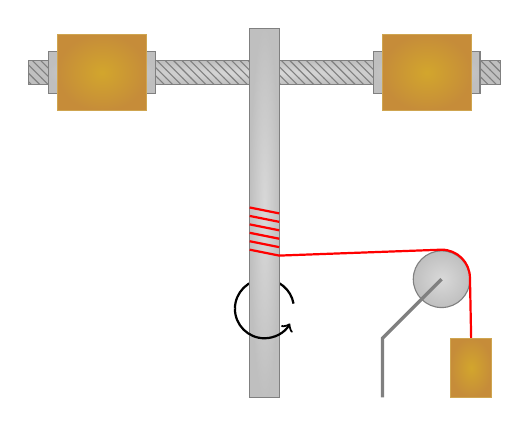
\begin{tikzpicture}
	[scale = 0.75,
	rod/.style={draw=gray,inner color = gray!30, outer color = gray!50},
	mass/.style={draw = yellow!20!brown, inner color = yellow!30!brown ,outer color = yellow!10!brown},
	string/.style = {thick, red}]
	\draw[thick] (-0.5,-4) arc (180:10:0.5);
	\fill [preaction={rod},pattern=north west lines, pattern color=gray] (-4,-0.2) rectangle (4,0.2);
	\fill [rod] (-0.25,0.75) rectangle (0.25,-5.5);
	\fill [rod] (3.65,-0.35) rectangle (1.85,0.35);
	\fill [rod] (-3.65,-0.35) rectangle (-1.85,0.35);
	\fill [mass] (3.5,-0.65) rectangle (2,0.65);
	\fill [mass] (-3.5,-0.65) rectangle (-2,0.65);
	\draw[thick, ->] (-0.5,-4) arc (180:330:0.5);
	\foreach \x in {0,...,5}
		\draw [string] (-0.25,\x/7-3) -- (0.25,\x/7-3.1);
	\draw [rod] (3,-3.5) circle (0.48);
	\draw [very thick, gray] (3,-3.5) -- (2,-4.5) -- (2,-5.5);
	\draw [string] (0.25,-3.1) -- (3,-3) arc (90:0:0.48) -- (3.5,-4.5);
	\draw [mass] (3.15,-4.5) rectangle (3.85,-5.5);
	\end{tikzpicture}
	\caption{As hanging mass is permitted to fall it causes the apparatus to begin spinning.}
\end{figure}

\section{Data}
\subsection{Constant Radius, Varying Masses}
As the mass was allowed to vary, the time required to fall the fixed distance was recorded a total of four times. For each trial, the time was recorded by hand with a simple stopwatch. Inevitably, there was variation in the recorded times for falling, and often one of the four trials would be significantly distant from the other three. Because of this, the value farthest from the mean was cast out and not used in the calculation of either of the mean or range of the time. The cast out values have been \emph{emphasized} in the data set in figures \ref{FIG:1} and \ref{FIG:2}.
\begin{figure}[h]
		\caption{Time Required to Fall function of Mass }
	\begin{center}
	\begin{tabular}{| c | c c c c | c | c |}
	\hline
	Masses & \multicolumn{4}{c|}{Measured Times} & Average Time & Time Range \\
	 (g) & \multicolumn{4}{c|}{(t)} & (t) & (t) \\
	\hline
	10 & 7.79 & \emph{8.00} & 7.82 & 7.82 & 7.81 & 0.03 \\ 
	20 & \emph{8.35} & 8.75 & 8.71 & 8.74 & 8.72 & 0.04 \\
	50 & 10.33 & 10.40 & \emph{10.05} & 10.48 & 10.40 & 0.15 \\ 
	100 & 12.61 & 12.63 & 12.83 & \emph{12.29} & 12.71 & 0.21 \\ 
	150 & 14.58 & 14.56 & \emph{14.50} & 14.55 & 14.56 & 0.03 \\ 
	200 & \emph{16.70} & 16.21 & 16.55 & 16.33 & 16.36 & 0.03 \\
	300 & 20.24 & 20.02 & 19.99 & \emph{20.37} & 20.08 & 0.25 \\  
	500 & 24.97 & 25.05 & \emph{25.25} & 25.09 & 25.04 & 0.12 \\
	\hline 
	\end{tabular}
	\end{center}
	\label{FIG:1}
\end{figure}
\subsection{Constant Mass, Varying Radius}
In the second series of measurements, rather than allowing the amount of mass on the spinning apparatus to vary, the distance at which the masses stood from the axis of rotation was varied. Again, the time required for the hanging mass to fall the fixed distance was measured a total of four times. And once again, the value farthest from the mean was \emph{cast out} and not used in the computation of the mean or range. 
\begin{figure}[h]
		\caption{Time Required to Fall function of Radius}
		\begin{center}
		\begin{tabular}{| c | c c c c | c | c |}
			\hline
			Distance & \multicolumn{4}{c|}{Measured Times} & Average Time & Time Range \\
			\hline
			3 & 8.20 & \emph{8.13} & 8.21 & 8.22 & 8.21 & 0.02 \\
			4 & 9.10 & \emph{8.95} & 9.02 & 9.06 & 9.06 & 0.08 \\
			5 & 10.08 & 10.08 & \emph{10.07} & 10.08 & 10.08 & 0.01 \\
			6 & 11.24 & 11.25 & \emph{11.06} & 11.31 & 11.27 & 0.07 \\
			7 & 12.32 & 12.38 & \emph{12.66} & 12.52 & 12.41 & 0.20 \\
			8 & 13.94 & \emph{13.78} & 13.85 & 13.93 & 13.90 & 0.08 \\
			9 & 15.11 & 15.03 & 15.16 & \emph{15.29} & 15.10 & 0.13 \\
			10 & 16.44 & 16.53 & \emph{16.43} & 16.53 & 16.50 & 0.09 \\
			11 & \emph{18.02} & 17.32 & 17.31 & 17.38 & 17.34 & 0.07 \\
			12 & 18.99 & 19.04 & 18.99 & \emph{18.62} & 19.01 & 0.05 \\
			13 & 20.63 & 20.64 & \emph{20.47} & 20.60 & 20.62 & 0.04 \\
			14 & 22.60 & 22.43 & 22.20 & \emph{21.98} & 22.41 & 0.4 \\
			15 & 23.35 & 23.36 & 23.44 & \emph{23.18} & 23.83 & 0.09 \\
			\hline 
		\end{tabular}
	\end{center}
\label{FIG:2}
\end{figure}
\subsection{Other Relevant Information}

\begin{figure}[h]
	\centering
	\caption{Other Relevant Measurements}
	\begin{tabular}{|c|c|}
		\hline
		Height of Fall & 88.35 \(\pm\) 0.1 cm \\
		\hline
		Diameter of Rod (Bare) & 1.27 \(\pm\) 0.01 cm \\
		\hline
		Diameter of Rod (With String) & 1.31 \(\pm\) 0.01 cm \\
		\hline
		Mass of Wing Nut & 6.04 \(\pm\) 0.03 g \\
		\hline
		Mass of Horizontal Rod & 62.19 \(\pm\) 0.02 g \\
		\hline
		Length of Horizontal Rod & 34.2 \(\pm\) 0.1 cm \\
		\hline       
		Local Gravitational Acceleration & 9.798 \( \pm \; 0.001 \; \textrm{m}/\textrm{s}^2 \)
		\\
		\hline
	\end{tabular}
\end{figure}
\section{Analysis}
\subsection{Finding Moment of Inertia}
One may compute the moment of inertia of the spinning apparatus as a function of the time required for the small hanging mass to fall. 
One may begin by first finding the tension in the string holding up the hanging mass. This tension is the force acting upon the rod and causing it to spin. Were the hanging mass, \(m\), to be at rest then the tension in the string would simply be the mass' weight \(m g\), however, the mass is indeed accelerating at some rate \(a\). This means the tension in the string is in fact smaller than the weight and in fact equal to the mass multiplied by the difference between the gravitational acceleration and the true acceleration of the mass.
\begin{equation}
F = m \left( g - a \right)
\end{equation}
This force is being applied on the vertical rod and causing it to spin. This force is inducing some angular acceleration into the rod and is hence causing some torque.
\begin{equation}
\tau = \vec{F} \times \vec{r}
\end{equation}
Because the tension in the string is acting tangent to the rod, the magnitude of the torque is simply equal to the product of the radius of the rod and the tension in the rope.
\begin{equation}
\tau = m r \left(g - a\right) \label{EQ:2}
\end{equation}
This torque causes an angular acceleration in the rods and masses proportional to the torque and inversely proportional to the moment of inertia of the spinning body
\begin{equation}
\alpha = \frac{\tau}{I}
\end{equation}
This angular acceleration is related to a linear acceleration of the string and hanging mass.
\begin{equation}
\alpha = \frac{a}{r}
\end{equation}
Combining the above two expressions allows one to write an expression for the moment of inertia function of the linear acceleration of the falling mass, torque acting on the rod, and radius of the rod.
\begin{equation}
I = \frac{\tau r}{a}
\end{equation}
One may then substitute the expression for torque as found in \eqref{EQ:2}.
\begin{equation}
I = \frac{m r^2 \left(g - a\right)}{a} \label{EQ:3}
\end{equation}
However, it is often difficult to accurately measure acceleration and because the acceleration in this system is constant it is sufficient to simply measure the time required to fall a fixed distance from rest. Recall that for bodies falling from rest the distance fallen, \(h\), may be written as a simple function of acceleration and time.
\begin{equation}
h = \frac{1}{2}a t^2
\end{equation}
One may rearrange this to find acceleration.
\begin{equation}
a = \frac{2 h}{t^2}
\end{equation}
If one substitutes this into equation \eqref{EQ:3} one may reach an expression for moment of inertia solely in terms of easily measurable quantities.
\begin{equation}
I = {\frac {m{r}^{2}{t}^{2}}{2h} \left( g-{\frac {2h}{{t}^{2}}}
	\right) }
\end{equation}
This simplifies to the somewhat more manageable expression.
\begin{equation}
I = {\frac {m{r}^{2} \left( g{t}^{2}-2\,h \right) }{2h}}
\end{equation}
\subsection{Errors In Moments of Inertia}
In order to find the quantity of error in the moment of inertia as a result of the error in each of the individual measurements in the experiments it is useful to find the derivatives of the moment of inertia with respect to each of the measurements. However, not all of the errors in measurements are significant enough to the create a large change in the moment of inertia. For example, both the mass of the hanging mass and the height of the table are known to within less than a tenth of a percent and hence will contribute rather little to the error in the calculated moment of inertia. In fact, only the time required to fall and the radius of the rod generate significant error. Fortunately both of these are relatively easy to differentiate.
\begin{equation}
\frac{\partial I }{\partial r} = \frac{2I}{r}
\end{equation}
\begin{equation}
\frac{\partial I }{\partial t} = \frac{2Itg}{g t^2-2 h}
\end{equation}
One may simply multiply these quantities by the estimated error in the respective quantities to find that particular measurements contribution to the error in the moment of inertia. If one assumes that the errors are uncorrelated the square estimated total error may be expressed as the sum of the square contributions from each of the measurements.
\section{Results and Conclusions}
\subsection{Interpretation of Results}
One may use the above expressions and the measured times to compute the moments of inertia of the apparatus in various positions.

One may begin to analyze the relations between the measured moment of inertia of the spinning apparatus and the additional masses placed on the horizontal threaded rod. If moment of inertia is truly a sum of products of mass and radius squared then, because the radius was kept constant in the first experiment, the relationship between mass and moment of inertia should appear to be linear.
\begin{figure}[h]
\centering
\caption{Measured Moment of Inertia Function of Additional Mass}
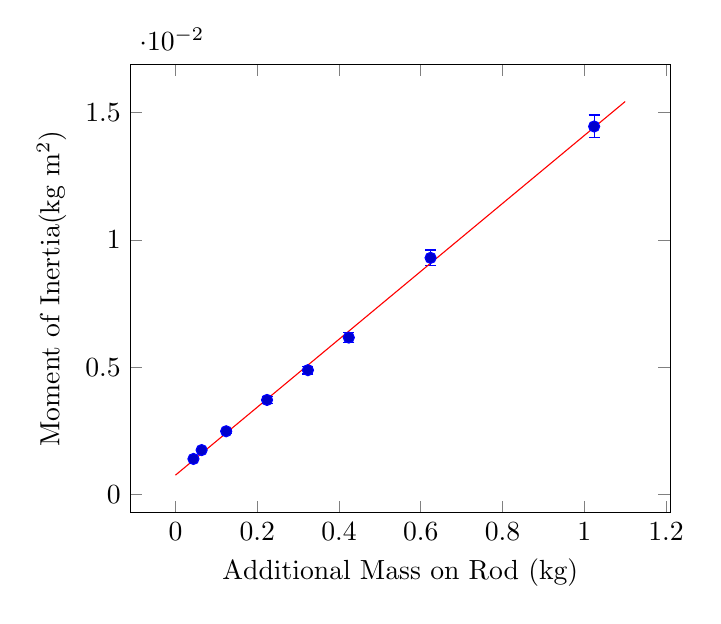
\begin{tikzpicture}
\begin{axis}[xlabel={Additional Mass on Rod (kg)},
 ylabel = {Moment of Inertia(kg \(\textrm{m}^2\))}]
	\addplot+[only marks,
	error bars/.cd,
	x dir=both,x explicit,
	y dir=both,y explicit,
	]
	table[x=x,y=y,,y error=yerror]
	{
		x      y        yerror
		0.044    0.001403 0.000044
		0.064    0.00175  0.000055
		0.124    0.00249  0.000085
		0.224    0.00372  0.00013
        0.324    0.00489  0.00015
        0.424    0.00617  0.00019 
        0.624    0.0093   0.00031
        1.024    0.01446   0.00045
	};
   \addplot[red,samples=100,domain=0:1.1] {0.01334*x+0.000766};
\end{axis}
\end{tikzpicture}
\end{figure}

This is, in fact, the relationship observed. Fitting a line to the dataset yields a remarkably close fit. So good of a fit that the \( \mathrm{R}^2 \) value is the remarkably high value of 0.9988. The particular curve yielded by the regression is \(I = 0.01334m + 0.000766\) However, there remain a few notable things about the linear regression. The first is its reluctance to pass through the origin. One might imagine that if there is no mass on the apparatus then the calculated moment of inertia ought to be zero as well. However, this is not the relationship suggested by the graph. The graphs suggestion is actually correct, even when there is no additional mass placed on the apparatus the two rods have mass and are positioned in such a way that they have a moment of inertia of their own. The y intercept of this curve,  \(7.66 \cdot 10^{-4} \pm 9 \cdot 10 ^{-6}  \; \mathrm{kg} \; \mathrm{m}^2 \), is an estimate for the moment of inertia of the bare system sans any additional mass. One might also wonder if the \(a\) parameter in the linear regression \(a\,x + b \) holds any significance. If moment of inertia of a point mass truly is of the form \(m \, r^2\) and the \(x\) parameter in our linear regression represents mass than one might predict that the \(a\) parameter is simply the square distance of the masses from the center of rotation. Or alternatively that the distance to the axis of rotation is simply the square root of this \(a\) term. One may compute that the square root of \(0.01334 \pm 0.0002 \; \mathrm{m}^2\) and yield the distance \(0.1155 \pm 0.0009 \mathrm{m}^2 \). This distance is relatively close to the true distance of the masses from the axis of rotation of \(10 \pm 0.1 \; \mathrm{cm}\)

One may conduct a similar analysis of the data in the second experiment. This time the data has a remarkably quadratic flair. A relationship which is reasonable given the expression for moment of inertia \(m \, r^2\).

\begin{figure}[h]
	\centering
	\caption{Measured Moment of Inertia Function of Distance of Additional Mass' Distance from Axis of Rotation}
	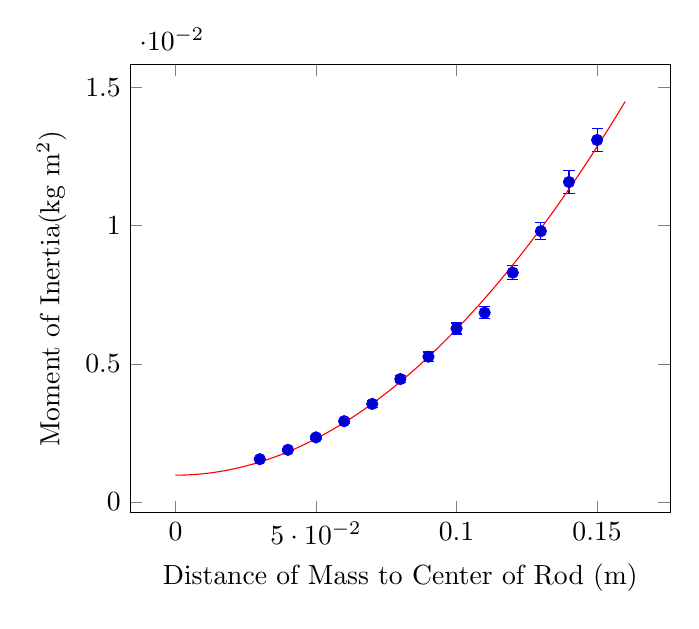
\begin{tikzpicture}
	\begin{axis}[xlabel={Distance of Mass to Center of Rod (m)},
	ylabel = {Moment of Inertia(kg \(\textrm{m}^2\))}]
	\addplot+[only marks,
	error bars/.cd,
	x dir=both,x explicit,
	y dir=both,y explicit,
	]
	table[x=x,y=y,,y error=yerror]
	{
		x      y        yerror
		0.03    0.001551  0.000048
		0.04    0.001889  0.000061
		0.05    0.00234   0.000074
		0.06    0.002926  0.000093
		0.07    0.00355   0.00012
		0.08    0.00445   0.00014
		0.09    0.00526   0.00017
		0.10    0.00628   0.0002
		0.11    0.00685   0.00021
		0.12    0.0083   0.00026
		0.13    0.0098   0.0003
		0.14    0.01158   0.00041 
		0.15    0.0131   0.00041
	};
	\addplot[red,samples=100,domain=0:0.16] {0.5281*x*x+0.000973};
	\end{axis}
	\end{tikzpicture}
\end{figure}
The equation for the best quadratic fit for this data is the curve \(I = 0.5281 r^2 + 0.00973\). And just as in the previous example, each of these parameters have a physical meaning. Again the y intercept of the function represents what would happen if the two masses were positioned directly on top of the axis of rotation. We have been treating the masses like point masses thus far, and if the masses were truly point masses then the y intercept would represent the moment of inertia of the bare apparatus. This particular experiments estimates the moment of inertia of the bare apparatus as  \(9 \cdot 10^{-4} \pm 2 \cdot 10 ^{-4}  \; \mathrm{kg} \; \mathrm{m}^2 \). The \(a\) portion of the expression \(a \; x^2 + c\) also has important physical meaning. Again, if one assumes that moment of inertia is truly \(m \; r^2 \) than the \(a\) value should simply represent the mass of the added mass. This would estimate the added mass to be \( 530 \pm 30 \; \mathrm{g} \) value that is reasonably close but decidedly larger than the true added mass of 424 g (two 200 g masses + four 6 gram wing nuts).
\subsection{An Analysis of Error}
One might attempt to compare the measured moments of inertia to an estimate of the moment of inertia using the geometry of the apparatus. The apparatus was composed of two rods one vertical and one horizontal. The horizontal rod spun perpendicular to its axis about its center. There is a simple expression for the moment of inertia of such a rod.
\begin{equation}
I = \frac{1}{12}\, m \, L^2
\end{equation}
Substituting the measured length of the rod, \(34.2 \pm 0.1 \mathrm{cm}\), and the measured mass of the rod, \(62.19 \pm 0.02 \, \mathrm{g} \) , yields the expression for moment of inertia, \(6.06 \cdot 10^{-4} \pm 3.6 \cdot 10^{-6} \mathrm{\, kg \, m}^2\). One might also consider the moment of inertia of the vertical rod which was much smaller. No direct measurements for the geometry of this rod were taken but estimates will be given. Because the small moment of inertia of the vertical rod even very rough estimate do not contribute greatly to error. The mass of the vertical rod was estimated to be \(200 \pm 100 \; \mathrm{g} \) and the radius was measured to be \(0.655 \pm 0.01 \; \mathrm{cm}\). Computation yields the vertical rod's contribution to moment of inertia to be the rather small value of \(4 \cdot 10^{-6} \pm 2 \cdot 10^{-6} \mathrm{\, kg \, m}^2\). Summing these two values shows that the moment of inertia, as nucleated by the physical geometry of the apparatus is estimated to be \(6.10 \cdot 10^{-4} \pm 4 \cdot 10^{-6} \mathrm{\, kg \, m}^2\).

Comparing this value to the measured moments of inertia shows that they serve as a reasonable estimate for the moment of inertia of the bare apparatus. The first intercept estimates the moment of inertia to be \(7.66 \cdot 10^{-4} \pm 9 \cdot 10 ^{-6}  \; \mathrm{kg} \; \mathrm{m}^2 \). There is a 25\%  error between the value that had been geometrically obtained and the value that has been obtained by measurements. However the error bars on each are terribly small. This suggests that some systematic error has caused either a systematic over estimation of the error on the part of the falling mass method or a systematic underestimation on the part of the geometric method. It is more to be likely the former of the two. Recall that in all the calculations the masses were treated as point masses. However in reality the masses have width and hence their moments of inertia are affected by that width. This effect causes the an overestimate as, because the radius is squared, the father away points make a greater contribution and hence pull the masses 'effective' center of mass father out. It is also work noting that the pulley used to suspend the string was not in the best of shape string would slip on the pulley as it turned. This friction would cause the hanging mass to take longer to fall and hence lead to an overestimate in the moment of inertia.

The second value is yet father away from the geometric model at \(9 \cdot 10^{-4} \pm 2 \cdot 10 ^{-4}  \; \mathrm{kg} \; \mathrm{m}^2 \) or nearly 50\% away. In this case both of the previously mentioned sources of error exist and contribute to the overestimate in moment of inertia. But there is yet another source of error. The y intercept of the function represents what would happen if the masses were placed at \(r = 0\). If they were a point mass this would be a representation of the bare apparatus, however the masses have width and thus their placement at the center would contribute to an increase in moment of inertia.

The same overestimates contribute to the 24\% overestimate in mass from the second experiment and the 11\% overestimate in the radius from the first experiment.


\end{document}